% This is a LaTeX template for poster using University of Helsinki style
% This version uses pdflatex; if you have XeTeX available, 
% consider using poster_xetex.tex for fancy font settings
%
% The official Graphical Instructions available from hy.logodomain.com (from university network only) defines colours, fonts etc. This Template does not perfectly match the official poster template of the university
%
% Jukka Suomela's collection of LaTeX tricks has been invaluable in building this template: http://cs.helsinki.fi/u/josuomel/latex/ 
%
% Original template by Janne Korhonen
% This file by Juha Karkkainen

% Encoding of this file is iso-8859-1 latin 1

\documentclass[a4paper]{article} % This actually makes poster of size A4, scale up when printing. Used text font size is a bit small for A1 poster, preferably use \small in that case 

% Misc. packages
\usepackage[T1]{fontenc}
\usepackage{url}
\usepackage{amsfonts}
\usepackage[absolute]{textpos}
\usepackage{amssymb}
\usepackage{amsmath} 
\usepackage{amsthm}

% Graphics stuff
\usepackage[usenames,dvipsnames]{color}
\usepackage{graphicx}


% My favourite macros
\newcommand{\N}{\mathbb{N}} %natural numbers
\newcommand{\Z}{\mathbb{Z}} %integers
\newcommand{\Q}{\mathbb{Q}} %rationals
\newcommand{\R}{\mathbb{R}} %reals

\newcommand{\G}{\mathcal{G}} % fancy G
\newcommand{\A}{\mathcal{A}} % fancy A
\newcommand{\bO}{\mathcal{O}} % fancy O

\newcommand{\eos}{\#}
\newcommand{\rank}{\textsc{rank}}


% enumitem for controlling enumerate and itemize environments; usefull for saving space
\usepackage{enumitem}


% Fonts
%
% Palantino - Helvetica - Courier.
% I haven't really spent time to figure out how to best match the official university style with latex font packages, as I use XeTex myself...
\usepackage{mathpazo}
\linespread{1.10}
\usepackage[scaled]{helvet}
\usepackage{courier}

% Colours
\definecolor{sciorange}{RGB}{252,163,17}
\definecolor{unigray}{RGB}{140,140,140}
\definecolor{first}{RGB}{180,30,10}
\definecolor{second}{RGB}{10,120,130}
\definecolor{new}{RGB}{190,50,10}
\definecolor{wavelet}{RGB}{70,140,220}
%\definecolor{improved}{RGB}{80,200,80}
\definecolor{improved}{RGB}{10,100,160}
\definecolor{prior}{RGB}{140,140,140}

% Textpos to manually position blocks of text on the page
\usepackage[absolute]{textpos}

% We define 1 mm grid for positioning the text blocks on the page
% The idea is to leave 10 mm marginals to all sides; the three text columns are 60 mm wide with 5 mm space between columns.
\setlength{\TPHorizModule}{1mm}
\setlength{\TPVertModule}{1mm}

% The origin is set to right below the main title; this means that main title blocks have negative y-coordinate. There is actually no good reason for this, I just happened to do this that way.
\textblockorigin{10mm}{48.5mm}


% parindent is set to zero, because it looks better in posters
% you could also add some space between paragraphs here, but I use manual vertical spaces in this sample
\setlength{\parindent}{0pt}


% Finally, the content
\begin{document}
\pagestyle{empty} % To get rid of page numbers and so


% ------------------------------------------------------------------------------------------------------------------------------
% Main title, University logo etc.

% If you need more space for the title or want the logo to be bigger, you need to adjust various parameters, as I did not bother to automate this yet
% Mainly, move the textblockorigin above down and adjust all the boxes here to be higher up.

% First, the University logo. The included flame.pdf is a copy of the official logo in vector format, so it is good for all sizes.
% Box starts 10 mm from the top
\begin{textblock}{95}(0,-38.5)

\includegraphics[width=22mm]{flame}
\end{textblock}	

% University - Faculty - Department
% Box starts 10 mm from the top
\begin{textblock}{95}(95,-38.5)
{\fontsize{8}{7}\selectfont\sffamily\color{unigray}
\hfill HELSINGIN YLIOPISTO

\hfill HELSINGFORS UNIVERSITET

\hfill UNIVERSITY OF HELSINKI

\color{sciorange}\hfill MATEMAATTIS-LUONNONTIETEELLINEN TIEDEKUNTA

\hfill MATEMATISK-NATURVETENSKAPLIGA FAKULTETEN

\hfill FACULTY OF SCIENCE % For some reason, the last line here gets messed up without extra spaces...


}
\end{textblock}


% Main title
% If you need two lines for the title, you need to adjust the position of this block and textblockorigin
% Remember, two first words use faculty colour. If your title is long, you can use small letters.
\begin{textblock}{190}(0,-13.5)
{\sffamily\LARGE{\color{sciorange}IMPROVING INVERSE }{\color{unigray}
BURROWS--WHEELER TRANSFORM\\THROUGHOUT THE SPACE--TIME SPECTRUM}}
\small\hfill Juha K\"arkk\"ainen and Simon Puglisi\\ % If you have multiple authors, their names can be on the same line. Adjust font size as necessary
\rule[2mm]{190mm}{0.3pt} % This is the line under the title, adjust the last parameter if it seems to be in the wrong place
\end{textblock}

% ------------------------- ABSTRACT ----------------------------------
% The "abstract" block. Does not actually exist in the university poster template, so you may consider not using this
\begin{textblock}{92.5}(0,0)
\sffamily
\small 
The Burrows-Wheeler transform (BWT) is a powerful tool for data
compression used for example in the popular compression program
bzip2. The \emph{inverse} BWT is usually the bottleneck in the
decompression phase with respect to both space and time.
\end{textblock}
\begin{textblock}{92.5}(97.5,0) 
  \sffamily \small 
  Our new algorithms improve the performance of inverse BWT.  They
  range from the fastest known algorithm to the most space-efficient
  one, and cover the whole space-time tradeoff spectrum in between.
\end{textblock}

% Large subtitle with line. Again, not from the university template.
%\begin{textblock}{190}(0,25)
%\sffamily
%\Large{\color{sciorange}ARITHMETIZATION}\small\\
%\rule[3mm]{190mm}{0.3pt}
%\end{textblock} 

% ---------------------------- INTRO ----------------------------------
% Three-column stuff
%
% The vertical size of the columns depends on the content, so unfortunately you have to manually move contents around

% First column
\begin{textblock}{60}(0,20)
  {\sffamily\normalsize{\color{sciorange}BURROWS--WHEELER
      TRANSFORM}}\vspace{1mm}\\ % Titles among the main text are made like this, not by using \section
  \footnotesize 
The Burrows--Wheeler transform (BWT) is an invertible text transform
defined as follows.\vspace{3mm}

{\scriptsize\sffamily
\quad{\bf Input: } text $T={}$BANANA\eos
\vspace{2mm}

\tabcolsep=.25em
\quad\begin{minipage}[t]{26mm}
\raggedright
%\centering
  1. Build a matrix with the text \emph{rotations} as rows
\begin{center}
\sffamily
    \begin{tabular}{ccccccc}
 %   \multicolumn{1}{c}{$F$} &&&&&\multicolumn{1}{c}{}& \multicolumn{1}{c}{}\\
    B&A&N&A&N&A&\eos\\
    A&N&A&N&A&\eos&B\\
    N&A&N&A&\eos&B&A\\
    A&N&A&\eos&B&A&N\\
    N&A&\eos&B&A&N&A\\
    A&\eos&B&A&N&A&N\\
    \eos&B&A&N&A&N&A\\
  \end{tabular}
  \end{center}
\end{minipage}
% \parbox[t]{6mm}{\centering \mbox{}\\\rule{0pt}{20mm}
% $\overset{\textrm{sort}}{\Rightarrow}$
% }%
\hfill
\begin{minipage}[t]{28mm}
\centering 2. Sort the rows
\begin{center}
\sffamily
    \begin{tabular}{|c|ccccc|c|}
    \multicolumn{1}{c}{$F$} &&&&&\multicolumn{1}{c}{}& \multicolumn{1}{c}{$L$}\\
    \cline{1-1}\cline{7-7}
    \eos&B&A&N&A&N&A\\
    A&\eos&B&A&N&A&N\\
    A&N&A&\eos&B&A&N\\
    A&N&A&N&A&\eos&B\\
    B&A&N&A&N&A&\eos\\
    N&A&\eos&B&A&N&A\\
    N&A&N&A&\eos&B&A\\
    \cline{1-1}\cline{7-7}
  \end{tabular}
\end{center}
\end{minipage}
\vspace{2mm}

\quad{\bf Output: } BWT $L={}$ANNB\eos AA (the last column)
\vspace{3mm}
}

\footnotesize The properties of the BWT make it easier to
compress than the original text. It is used as the first stage in many
compression programs including the widely used bzip2 (thus the b).

\end{textblock} 

% Second column
\begin{textblock}{60}(65,20)
  {\sffamily\normalsize{\color{sciorange}INVERSE BWT}}\vspace{1mm}\\
  \footnotesize 
  Define
  $
    \rank(j)=\big|\{i \mid i<j \textrm{ and }
    L[i]=L[j]\}\big|.
  $

The BWT can be inverted as follows.
\vspace{3mm}

\scriptsize\sffamily
\quad{\bf Input: } BWT $L={}$ANNB\eos AA
\vspace{2mm}

\quad\begin{minipage}{55mm}
\scriptsize\sffamily
1. Compute $C$ and \rank\ arrays by scanning $L$
\scriptsize\sffamily
\begin{center}
\hspace*{-5mm}\begin{picture}(0,0)%
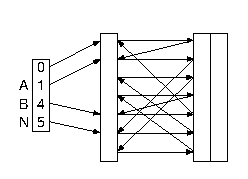
\includegraphics{./permutation}%
\end{picture}%
\setlength{\unitlength}{2983sp}%
%
\begingroup\makeatletter\ifx\SetFigFont\undefined%
\gdef\SetFigFont#1#2#3#4#5{%
  \reset@font\fontsize{#1}{#2pt}%
  \fontfamily{#3}\fontseries{#4}\fontshape{#5}%
  \selectfont}%
\fi\endgroup%
\begin{picture}(2249,1542)(329,-1648)
\put(1306,-241){\makebox(0,0)[b]{\smash{{\SetFigFont{7}{8.4}{\sfdefault}{\mddefault}{\updefault}{\color[rgb]{0,0,0}$F$}%
}}}}
\put(1306,-421){\makebox(0,0)[b]{\smash{{\SetFigFont{7}{8.4}{\sfdefault}{\mddefault}{\updefault}{\color[rgb]{0,0,0}\eos}%
}}}}
\put(1306,-616){\makebox(0,0)[b]{\smash{{\SetFigFont{7}{8.4}{\sfdefault}{\mddefault}{\updefault}{\color[rgb]{0,0,0}A}%
}}}}
\put(1306,-811){\makebox(0,0)[b]{\smash{{\SetFigFont{7}{8.4}{\sfdefault}{\mddefault}{\updefault}{\color[rgb]{0,0,0}A}%
}}}}
\put(1306,-1201){\makebox(0,0)[b]{\smash{{\SetFigFont{7}{8.4}{\sfdefault}{\mddefault}{\updefault}{\color[rgb]{0,0,0}B}%
}}}}
\put(1306,-1396){\makebox(0,0)[b]{\smash{{\SetFigFont{7}{8.4}{\sfdefault}{\mddefault}{\updefault}{\color[rgb]{0,0,0}N}%
}}}}
\put(1306,-1591){\makebox(0,0)[b]{\smash{{\SetFigFont{7}{8.4}{\sfdefault}{\mddefault}{\updefault}{\color[rgb]{0,0,0}N}%
}}}}
\put(1306,-1006){\makebox(0,0)[b]{\smash{{\SetFigFont{7}{8.4}{\sfdefault}{\mddefault}{\updefault}{\color[rgb]{0,0,0}A}%
}}}}
\put(2296,-241){\makebox(0,0)[b]{\smash{{\SetFigFont{7}{8.4}{\sfdefault}{\mddefault}{\updefault}{\color[rgb]{0,0,0}$L$}%
}}}}
\put(2296,-616){\makebox(0,0)[b]{\smash{{\SetFigFont{7}{8.4}{\sfdefault}{\mddefault}{\updefault}{\color[rgb]{0,0,0}N}%
}}}}
\put(2296,-811){\makebox(0,0)[b]{\smash{{\SetFigFont{7}{8.4}{\sfdefault}{\mddefault}{\updefault}{\color[rgb]{0,0,0}N}%
}}}}
\put(2296,-1006){\makebox(0,0)[b]{\smash{{\SetFigFont{7}{8.4}{\sfdefault}{\mddefault}{\updefault}{\color[rgb]{0,0,0}B}%
}}}}
\put(2296,-1201){\makebox(0,0)[b]{\smash{{\SetFigFont{7}{8.4}{\sfdefault}{\mddefault}{\updefault}{\color[rgb]{0,0,0}\eos}%
}}}}
\put(2296,-1396){\makebox(0,0)[b]{\smash{{\SetFigFont{7}{8.4}{\sfdefault}{\mddefault}{\updefault}{\color[rgb]{0,0,0}A}%
}}}}
\put(2296,-1591){\makebox(0,0)[b]{\smash{{\SetFigFont{7}{8.4}{\sfdefault}{\mddefault}{\updefault}{\color[rgb]{0,0,0}A}%
}}}}
\put(2296,-421){\makebox(0,0)[b]{\smash{{\SetFigFont{7}{8.4}{\sfdefault}{\mddefault}{\updefault}{\color[rgb]{0,0,0}A}%
}}}}
\put(586,-511){\makebox(0,0)[b]{\smash{{\SetFigFont{7}{8.4}{\sfdefault}{\mddefault}{\updefault}{\color[rgb]{0,0,0}$C$}%
}}}}
\put(406,-691){\makebox(0,0)[b]{\smash{{\SetFigFont{7}{8.4}{\sfdefault}{\mddefault}{\updefault}{\color[rgb]{0,0,0}\eos}%
}}}}
\put(2476,-421){\makebox(0,0)[b]{\smash{{\SetFigFont{7}{8.4}{\sfdefault}{\mddefault}{\updefault}{\color[rgb]{0,0,0}0}%
}}}}
\put(2476,-616){\makebox(0,0)[b]{\smash{{\SetFigFont{7}{8.4}{\sfdefault}{\mddefault}{\updefault}{\color[rgb]{0,0,0}0}%
}}}}
\put(2476,-811){\makebox(0,0)[b]{\smash{{\SetFigFont{7}{8.4}{\sfdefault}{\mddefault}{\updefault}{\color[rgb]{0,0,0}1}%
}}}}
\put(2476,-1006){\makebox(0,0)[b]{\smash{{\SetFigFont{7}{8.4}{\sfdefault}{\mddefault}{\updefault}{\color[rgb]{0,0,0}0}%
}}}}
\put(2476,-1201){\makebox(0,0)[b]{\smash{{\SetFigFont{7}{8.4}{\sfdefault}{\mddefault}{\updefault}{\color[rgb]{0,0,0}0}%
}}}}
\put(2476,-1396){\makebox(0,0)[b]{\smash{{\SetFigFont{7}{8.4}{\sfdefault}{\mddefault}{\updefault}{\color[rgb]{0,0,0}1}%
}}}}
\put(2476,-1591){\makebox(0,0)[b]{\smash{{\SetFigFont{7}{8.4}{\sfdefault}{\mddefault}{\updefault}{\color[rgb]{0,0,0}2}%
}}}}
\put(2386,-241){\makebox(0,0)[lb]{\smash{{\SetFigFont{7}{8.4}{\sfdefault}{\mddefault}{\updefault}{\color[rgb]{0,0,0}$\rank$}%
}}}}
\end{picture}%
  
\end{center}
2. Starting at $L[i]={}$\eos, follow the permutation:
\[
i \mapsto C[L[i]]+\rank(i)
\]
\hspace{2.3mm}Output $L[i]$ at each step
\end{minipage}
\vspace{2mm}

\scriptsize\sffamily
\quad{\bf Output: } reverse text $T^R={}$\eos ANANAB

\end{textblock}


% ----------------------- ALGORITHMS ----------------------------

\begin{textblock}{125}(0,97)
\sffamily\normalsize{\color{sciorange}NEW ALGORITHMS FOR INVERSE BWT}\small\\
\rule[3mm]{125mm}{0.1pt}
\end{textblock} 


\begin{textblock}{60}(0,103) 
  \footnotesize 
  The basic inversion algorithm described above has linear time and
  space complexity, but it still dominates the time and space
  requirements during decompression in programs like bzip2.
  \vspace{1mm}

  It is slow because each memory access during the permutation 
  traversal is essentially random causing many cache misses.
  \vspace{1mm}

  It needs a lot of space for the \rank\ array:
  \begin{align*}
    |\rank| &= n\log n \textrm{ bits} = 4n \textrm{ bytes}\\[-1mm]
    |\textrm{text}| &= n\log\sigma \textrm{ bits} = n \textrm{ bytes}
  \end{align*}
  where $n={}$text length and $\sigma={}$alphabet size.
\end{textblock}

\begin{textblock}{60}(0,152)
  {\sffamily\normalsize{\color{sciorange}
      REFERENCE POINT RANKS}}\vspace{1mm}\\
  \footnotesize 
  We reduce space by storing ranks relative to reference points,
  which can be placed in two ways:\\

  \begin{minipage}[t]{25mm}
    \scriptsize\sffamily
    \centering
    Every $k$th position~\cite{ll2005}
    \begin{center}
      \begin{picture}(0,0)%
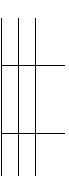
\includegraphics{./LR-B}%
\end{picture}%
\setlength{\unitlength}{2983sp}%
%
\begingroup\makeatletter\ifx\SetFigFont\undefined%
\gdef\SetFigFont#1#2#3#4#5{%
  \reset@font\fontsize{#1}{#2pt}%
  \fontfamily{#3}\fontseries{#4}\fontshape{#5}%
  \selectfont}%
\fi\endgroup%
\begin{picture}(710,1857)(2284,-1828)
\put(2566,-421){\makebox(0,0)[b]{\smash{{\SetFigFont{7}{8.4}{\sfdefault}{\mddefault}{\updefault}{\color[rgb]{0,0,0}1}%
}}}}
\put(2791,-601){\makebox(0,0)[b]{\smash{{\SetFigFont{7}{8.4}{\sfdefault}{\mddefault}{\updefault}{\color[rgb]{0,0,0}A}%
}}}}
\put(2926,-601){\makebox(0,0)[b]{\smash{{\SetFigFont{7}{8.4}{\sfdefault}{\mddefault}{\updefault}{\color[rgb]{0,0,0}B}%
}}}}
\put(2566,-601){\makebox(0,0)[b]{\smash{{\SetFigFont{7}{8.4}{\sfdefault}{\mddefault}{\updefault}{\color[rgb]{0,0,0}1}%
}}}}
\put(2566,-781){\makebox(0,0)[b]{\smash{{\SetFigFont{7}{8.4}{\sfdefault}{\mddefault}{\updefault}{\color[rgb]{0,0,0}0}%
}}}}
\put(2566,-961){\makebox(0,0)[b]{\smash{{\SetFigFont{7}{8.4}{\sfdefault}{\mddefault}{\updefault}{\color[rgb]{0,0,0}0}%
}}}}
\put(2566,-1141){\makebox(0,0)[b]{\smash{{\SetFigFont{7}{8.4}{\sfdefault}{\mddefault}{\updefault}{\color[rgb]{0,0,0}1}%
}}}}
\put(2566,-1321){\makebox(0,0)[b]{\smash{{\SetFigFont{7}{8.4}{\sfdefault}{\mddefault}{\updefault}{\color[rgb]{0,0,0}2}%
}}}}
\put(2791,-781){\makebox(0,0)[b]{\smash{{\SetFigFont{7}{8.4}{\sfdefault}{\mddefault}{\updefault}{\color[rgb]{0,0,0}4}%
}}}}
\put(2791,-1501){\makebox(0,0)[b]{\smash{{\SetFigFont{7}{8.4}{\sfdefault}{\mddefault}{\updefault}{\color[rgb]{0,0,0}7}%
}}}}
\put(2791,-1321){\makebox(0,0)[b]{\smash{{\SetFigFont{7}{8.4}{\sfdefault}{\mddefault}{\updefault}{\color[rgb]{0,0,0}A}%
}}}}
\put(2926,-1321){\makebox(0,0)[b]{\smash{{\SetFigFont{7}{8.4}{\sfdefault}{\mddefault}{\updefault}{\color[rgb]{0,0,0}B}%
}}}}
\put(2566,-1501){\makebox(0,0)[b]{\smash{{\SetFigFont{7}{8.4}{\sfdefault}{\mddefault}{\updefault}{\color[rgb]{0,0,0}0}%
}}}}
\put(2926,-1501){\makebox(0,0)[b]{\smash{{\SetFigFont{7}{8.4}{\sfdefault}{\mddefault}{\updefault}{\color[rgb]{0,0,0}5}%
}}}}
\put(2566,-1681){\makebox(0,0)[b]{\smash{{\SetFigFont{7}{8.4}{\sfdefault}{\mddefault}{\updefault}{\color[rgb]{0,0,0}1}%
}}}}
\put(2386,-106){\makebox(0,0)[b]{\smash{{\SetFigFont{7}{8.4}{\sfdefault}{\mddefault}{\updefault}{\color[rgb]{0,0,0}$L$}%
}}}}
\put(2386,-421){\makebox(0,0)[b]{\smash{{\SetFigFont{7}{8.4}{\sfdefault}{\mddefault}{\updefault}{\color[rgb]{0,0,0}A}%
}}}}
\put(2386,-601){\makebox(0,0)[b]{\smash{{\SetFigFont{7}{8.4}{\sfdefault}{\mddefault}{\updefault}{\color[rgb]{0,0,0}B}%
}}}}
\put(2386,-781){\makebox(0,0)[b]{\smash{{\SetFigFont{7}{8.4}{\sfdefault}{\mddefault}{\updefault}{\color[rgb]{0,0,0}A}%
}}}}
\put(2386,-961){\makebox(0,0)[b]{\smash{{\SetFigFont{7}{8.4}{\sfdefault}{\mddefault}{\updefault}{\color[rgb]{0,0,0}B}%
}}}}
\put(2386,-1141){\makebox(0,0)[b]{\smash{{\SetFigFont{7}{8.4}{\sfdefault}{\mddefault}{\updefault}{\color[rgb]{0,0,0}A}%
}}}}
\put(2386,-1321){\makebox(0,0)[b]{\smash{{\SetFigFont{7}{8.4}{\sfdefault}{\mddefault}{\updefault}{\color[rgb]{0,0,0}A}%
}}}}
\put(2386,-1501){\makebox(0,0)[b]{\smash{{\SetFigFont{7}{8.4}{\sfdefault}{\mddefault}{\updefault}{\color[rgb]{0,0,0}A}%
}}}}
\put(2386,-1681){\makebox(0,0)[b]{\smash{{\SetFigFont{7}{8.4}{\sfdefault}{\mddefault}{\updefault}{\color[rgb]{0,0,0}A}%
}}}}
\put(2926,-781){\makebox(0,0)[b]{\smash{{\SetFigFont{7}{8.4}{\sfdefault}{\mddefault}{\updefault}{\color[rgb]{0,0,0}4}%
}}}}
\put(2476,-106){\makebox(0,0)[lb]{\smash{{\SetFigFont{7}{8.4}{\sfdefault}{\mddefault}{\updefault}{\color[rgb]{0,0,0}$\rank$}%
}}}}
\end{picture}%

    \end{center}
  \end{minipage}
  \hfill
  \begin{minipage}[t]{30mm}
    \scriptsize\sffamily
    \centering
    Every $k$th occurrence [new]
    \begin{center}
      \begin{picture}(0,0)%

\includegraphics{./LR-I}%
\end{picture}%
\setlength{\unitlength}{2983sp}%
%
\begingroup\makeatletter\ifx\SetFigFont\undefined%
\gdef\SetFigFont#1#2#3#4#5{%
  \reset@font\fontsize{#1}{#2pt}%
  \fontfamily{#3}\fontseries{#4}\fontshape{#5}%
  \selectfont}%
\fi\endgroup%
\begin{picture}(1565,1857)(1693,-1828)
\put(3151,-1051){\makebox(0,0)[b]{\smash{{\SetFigFont{7}{8.4}{\sfdefault}{\mddefault}{\updefault}{\color[rgb]{0,0,0}8}%
}}}}
\put(3151,-1231){\makebox(0,0)[b]{\smash{{\SetFigFont{7}{8.4}{\sfdefault}{\mddefault}{\updefault}{\color[rgb]{0,0,0}12}%
}}}}
\put(3151,-646){\makebox(0,0)[b]{\smash{{\SetFigFont{7}{8.4}{\sfdefault}{\mddefault}{\updefault}{\color[rgb]{0,0,0}A}%
}}}}
\put(3151,-871){\makebox(0,0)[b]{\smash{{\SetFigFont{7}{8.4}{\sfdefault}{\mddefault}{\updefault}{\color[rgb]{0,0,0}4}%
}}}}
\put(2566,-421){\makebox(0,0)[b]{\smash{{\SetFigFont{7}{8.4}{\sfdefault}{\mddefault}{\updefault}{\color[rgb]{0,0,0}3}%
}}}}
\put(2566,-601){\makebox(0,0)[b]{\smash{{\SetFigFont{7}{8.4}{\sfdefault}{\mddefault}{\updefault}{\color[rgb]{0,0,0}3}%
}}}}
\put(2566,-781){\makebox(0,0)[b]{\smash{{\SetFigFont{7}{8.4}{\sfdefault}{\mddefault}{\updefault}{\color[rgb]{0,0,0}0}%
}}}}
\put(2566,-961){\makebox(0,0)[b]{\smash{{\SetFigFont{7}{8.4}{\sfdefault}{\mddefault}{\updefault}{\color[rgb]{0,0,0}0}%
}}}}
\put(2566,-1141){\makebox(0,0)[b]{\smash{{\SetFigFont{7}{8.4}{\sfdefault}{\mddefault}{\updefault}{\color[rgb]{0,0,0}1}%
}}}}
\put(2566,-1321){\makebox(0,0)[b]{\smash{{\SetFigFont{7}{8.4}{\sfdefault}{\mddefault}{\updefault}{\color[rgb]{0,0,0}2}%
}}}}
\put(2566,-1501){\makebox(0,0)[b]{\smash{{\SetFigFont{7}{8.4}{\sfdefault}{\mddefault}{\updefault}{\color[rgb]{0,0,0}3}%
}}}}
\put(2566,-1681){\makebox(0,0)[b]{\smash{{\SetFigFont{7}{8.4}{\sfdefault}{\mddefault}{\updefault}{\color[rgb]{0,0,0}0}%
}}}}
\put(1801,-1051){\makebox(0,0)[b]{\smash{{\SetFigFont{7}{8.4}{\sfdefault}{\mddefault}{\updefault}{\color[rgb]{0,0,0}8}%
}}}}
\put(1801,-1231){\makebox(0,0)[b]{\smash{{\SetFigFont{7}{8.4}{\sfdefault}{\mddefault}{\updefault}{\color[rgb]{0,0,0}12}%
}}}}
\put(1801,-646){\makebox(0,0)[b]{\smash{{\SetFigFont{7}{8.4}{\sfdefault}{\mddefault}{\updefault}{\color[rgb]{0,0,0}B}%
}}}}
\put(1801,-871){\makebox(0,0)[b]{\smash{{\SetFigFont{7}{8.4}{\sfdefault}{\mddefault}{\updefault}{\color[rgb]{0,0,0}4}%
}}}}
\put(2386,-106){\makebox(0,0)[b]{\smash{{\SetFigFont{7}{8.4}{\sfdefault}{\mddefault}{\updefault}{\color[rgb]{0,0,0}$L$}%
}}}}
\put(2386,-421){\makebox(0,0)[b]{\smash{{\SetFigFont{7}{8.4}{\sfdefault}{\mddefault}{\updefault}{\color[rgb]{0,0,0}A}%
}}}}
\put(2386,-601){\makebox(0,0)[b]{\smash{{\SetFigFont{7}{8.4}{\sfdefault}{\mddefault}{\updefault}{\color[rgb]{0,0,0}B}%
}}}}
\put(2386,-781){\makebox(0,0)[b]{\smash{{\SetFigFont{7}{8.4}{\sfdefault}{\mddefault}{\updefault}{\color[rgb]{0,0,0}A}%
}}}}
\put(2386,-961){\makebox(0,0)[b]{\smash{{\SetFigFont{7}{8.4}{\sfdefault}{\mddefault}{\updefault}{\color[rgb]{0,0,0}B}%
}}}}
\put(2386,-1141){\makebox(0,0)[b]{\smash{{\SetFigFont{7}{8.4}{\sfdefault}{\mddefault}{\updefault}{\color[rgb]{0,0,0}A}%
}}}}
\put(2386,-1321){\makebox(0,0)[b]{\smash{{\SetFigFont{7}{8.4}{\sfdefault}{\mddefault}{\updefault}{\color[rgb]{0,0,0}A}%
}}}}
\put(2386,-1501){\makebox(0,0)[b]{\smash{{\SetFigFont{7}{8.4}{\sfdefault}{\mddefault}{\updefault}{\color[rgb]{0,0,0}A}%
}}}}
\put(2386,-1681){\makebox(0,0)[b]{\smash{{\SetFigFont{7}{8.4}{\sfdefault}{\mddefault}{\updefault}{\color[rgb]{0,0,0}A}%
}}}}
\put(2476,-106){\makebox(0,0)[lb]{\smash{{\SetFigFont{7}{8.4}{\sfdefault}{\mddefault}{\updefault}{\color[rgb]{0,0,0}$\rank$}%
}}}}
\end{picture}%

    \end{center}
  \end{minipage}
  \vspace{3mm}

  \begin{minipage}{42mm}
%\scriptsize\sffamily
%\centering
    \raggedright
    A new improvement is to use variable length encoding, where
    a frequent symbol uses less bits for symbol and more bits for rank.
  \end{minipage}
  \hfill
  \begin{minipage}{17mm}
    \begin{center}
      \begin{picture}(0,0)%

\includegraphics{./variable}%
\end{picture}%
\setlength{\unitlength}{2983sp}%
%
\begingroup\makeatletter\ifx\SetFigFont\undefined%
\gdef\SetFigFont#1#2#3#4#5{%
  \reset@font\fontsize{#1}{#2pt}%
  \fontfamily{#3}\fontseries{#4}\fontshape{#5}%
  \selectfont}%
\fi\endgroup%
\begin{picture}(384,1002)(2284,-1333)
\put(2362,-1141){\makebox(0,0)[b]{\smash{{\SetFigFont{7}{8.4}{\sfdefault}{\mddefault}{\updefault}{\color[rgb]{0,0,0}A}%
}}}}
\put(2408,-965){\makebox(0,0)[b]{\smash{{\SetFigFont{7}{8.4}{\sfdefault}{\mddefault}{\updefault}{\color[rgb]{0,0,0}B}%
}}}}
\put(2359,-777){\makebox(0,0)[b]{\smash{{\SetFigFont{7}{8.4}{\sfdefault}{\mddefault}{\updefault}{\color[rgb]{0,0,0}A}%
}}}}
\put(2550,-781){\makebox(0,0)[b]{\smash{{\SetFigFont{7}{8.4}{\sfdefault}{\mddefault}{\updefault}{\color[rgb]{0,0,0}0}%
}}}}
\put(2593,-961){\makebox(0,0)[b]{\smash{{\SetFigFont{7}{8.4}{\sfdefault}{\mddefault}{\updefault}{\color[rgb]{0,0,0}0}%
}}}}
\put(2547,-1145){\makebox(0,0)[b]{\smash{{\SetFigFont{7}{8.4}{\sfdefault}{\mddefault}{\updefault}{\color[rgb]{0,0,0}1}%
}}}}
\put(2386,-466){\makebox(0,0)[b]{\smash{{\SetFigFont{7}{8.4}{\sfdefault}{\mddefault}{\updefault}{\color[rgb]{0,0,0}$L$}%
}}}}
\put(2476,-466){\makebox(0,0)[lb]{\smash{{\SetFigFont{7}{8.4}{\sfdefault}{\mddefault}{\updefault}{\color[rgb]{0,0,0}$\rank$}%
}}}}
\end{picture}%

    \end{center}
  \end{minipage}
  \vspace{1mm}

  Finally, we can trade time for space by replacing \rank\ with
  scanning from the nearest reference point~\cite{ll2005}.
\end{textblock}

\begin{textblock}{60}(65,104) 
  {\sffamily\normalsize{\color{sciorange}
      REPETITION SHORTCUTS}}\vspace{1mm}\\
  \footnotesize 
  Repetitions in the text manifest as \emph{pairs of parallel paths}
  (PPP) in the inverse BWT permutation. We use this as follows.
  \vspace{3mm}

  \begin{minipage}[t]{29mm}
    \scriptsize\sffamily
    \centering
    1. On the {\color{first}first pass},\\observe the PPP\\
    (due to repeated ANA)
    \begin{center}
      \begin{picture}(0,0)%

\includegraphics{./copy1}%
\end{picture}%
\setlength{\unitlength}{2983sp}%
%
\begingroup\makeatletter\ifx\SetFigFont\undefined%
\gdef\SetFigFont#1#2#3#4#5{%
  \reset@font\fontsize{#1}{#2pt}%
  \fontfamily{#3}\fontseries{#4}\fontshape{#5}%
  \selectfont}%
\fi\endgroup%
\begin{picture}(1194,1542)(1204,-1648)
\put(2296,-241){\makebox(0,0)[b]{\smash{{\SetFigFont{7}{8.4}{\sfdefault}{\mddefault}{\updefault}{\color[rgb]{0,0,0}$L$}%
}}}}
\put(2296,-616){\makebox(0,0)[b]{\smash{{\SetFigFont{7}{8.4}{\sfdefault}{\mddefault}{\updefault}{\color[rgb]{0,0,0}N}%
}}}}
\put(2296,-811){\makebox(0,0)[b]{\smash{{\SetFigFont{7}{8.4}{\sfdefault}{\mddefault}{\updefault}{\color[rgb]{0,0,0}N}%
}}}}
\put(2296,-1006){\makebox(0,0)[b]{\smash{{\SetFigFont{7}{8.4}{\sfdefault}{\mddefault}{\updefault}{\color[rgb]{0,0,0}B}%
}}}}
\put(2296,-1201){\makebox(0,0)[b]{\smash{{\SetFigFont{7}{8.4}{\sfdefault}{\mddefault}{\updefault}{\color[rgb]{0,0,0}\eos}%
}}}}
\put(2296,-1396){\makebox(0,0)[b]{\smash{{\SetFigFont{7}{8.4}{\sfdefault}{\mddefault}{\updefault}{\color[rgb]{0,0,0}A}%
}}}}
\put(2296,-1591){\makebox(0,0)[b]{\smash{{\SetFigFont{7}{8.4}{\sfdefault}{\mddefault}{\updefault}{\color[rgb]{0,0,0}A}%
}}}}
\put(2296,-421){\makebox(0,0)[b]{\smash{{\SetFigFont{7}{8.4}{\sfdefault}{\mddefault}{\updefault}{\color[rgb]{0,0,0}A}%
}}}}
\put(1306,-241){\makebox(0,0)[b]{\smash{{\SetFigFont{7}{8.4}{\sfdefault}{\mddefault}{\updefault}{\color[rgb]{0,0,0}$F$}%
}}}}
\put(1306,-421){\makebox(0,0)[b]{\smash{{\SetFigFont{7}{8.4}{\sfdefault}{\mddefault}{\updefault}{\color[rgb]{0,0,0}\eos}%
}}}}
\put(1306,-616){\makebox(0,0)[b]{\smash{{\SetFigFont{7}{8.4}{\sfdefault}{\mddefault}{\updefault}{\color[rgb]{0,0,0}A}%
}}}}
\put(1306,-811){\makebox(0,0)[b]{\smash{{\SetFigFont{7}{8.4}{\sfdefault}{\mddefault}{\updefault}{\color[rgb]{0,0,0}A}%
}}}}
\put(1306,-1201){\makebox(0,0)[b]{\smash{{\SetFigFont{7}{8.4}{\sfdefault}{\mddefault}{\updefault}{\color[rgb]{0,0,0}B}%
}}}}
\put(1306,-1396){\makebox(0,0)[b]{\smash{{\SetFigFont{7}{8.4}{\sfdefault}{\mddefault}{\updefault}{\color[rgb]{0,0,0}N}%
}}}}
\put(1306,-1591){\makebox(0,0)[b]{\smash{{\SetFigFont{7}{8.4}{\sfdefault}{\mddefault}{\updefault}{\color[rgb]{0,0,0}N}%
}}}}
\put(1306,-1006){\makebox(0,0)[b]{\smash{{\SetFigFont{7}{8.4}{\sfdefault}{\mddefault}{\updefault}{\color[rgb]{0,0,0}A}%
}}}}
\end{picture}%

    \end{center}
  \end{minipage}
  \hfill
  \begin{minipage}[t]{29mm}
    \scriptsize\sffamily
    \centering
    2. Replace the {\color{second}other path} by shortcut and
    follow it\\on the second pass
    \begin{center}
      \begin{picture}(0,0)%

\includegraphics{./copy2}%
\end{picture}%
\setlength{\unitlength}{2983sp}%
%
\begingroup\makeatletter\ifx\SetFigFont\undefined%
\gdef\SetFigFont#1#2#3#4#5{%
  \reset@font\fontsize{#1}{#2pt}%
  \fontfamily{#3}\fontseries{#4}\fontshape{#5}%
  \selectfont}%
\fi\endgroup%
\begin{picture}(1374,1542)(1204,-1648)
\put(2296,-241){\makebox(0,0)[b]{\smash{{\SetFigFont{7}{8.4}{\sfdefault}{\mddefault}{\updefault}{\color[rgb]{0,0,0}$L$}%
}}}}
\put(2296,-616){\makebox(0,0)[b]{\smash{{\SetFigFont{7}{8.4}{\sfdefault}{\mddefault}{\updefault}{\color[rgb]{0,0,0}N}%
}}}}
\put(2296,-811){\makebox(0,0)[b]{\smash{{\SetFigFont{7}{8.4}{\sfdefault}{\mddefault}{\updefault}{\color[rgb]{0,0,0}N}%
}}}}
\put(2296,-1006){\makebox(0,0)[b]{\smash{{\SetFigFont{7}{8.4}{\sfdefault}{\mddefault}{\updefault}{\color[rgb]{0,0,0}B}%
}}}}
\put(2296,-1201){\makebox(0,0)[b]{\smash{{\SetFigFont{7}{8.4}{\sfdefault}{\mddefault}{\updefault}{\color[rgb]{0,0,0}\eos}%
}}}}
\put(2296,-1396){\makebox(0,0)[b]{\smash{{\SetFigFont{7}{8.4}{\sfdefault}{\mddefault}{\updefault}{\color[rgb]{0,0,0}A}%
}}}}
\put(2296,-1591){\makebox(0,0)[b]{\smash{{\SetFigFont{7}{8.4}{\sfdefault}{\mddefault}{\updefault}{\color[rgb]{0,0,0}A}%
}}}}
\put(2296,-421){\makebox(0,0)[b]{\smash{{\SetFigFont{7}{8.4}{\sfdefault}{\mddefault}{\updefault}{\color[rgb]{0,0,0}A}%
}}}}
\put(1306,-241){\makebox(0,0)[b]{\smash{{\SetFigFont{7}{8.4}{\sfdefault}{\mddefault}{\updefault}{\color[rgb]{0,0,0}$F$}%
}}}}
\put(1306,-421){\makebox(0,0)[b]{\smash{{\SetFigFont{7}{8.4}{\sfdefault}{\mddefault}{\updefault}{\color[rgb]{0,0,0}\eos}%
}}}}
\put(1306,-616){\makebox(0,0)[b]{\smash{{\SetFigFont{7}{8.4}{\sfdefault}{\mddefault}{\updefault}{\color[rgb]{0,0,0}A}%
}}}}
\put(1306,-811){\makebox(0,0)[b]{\smash{{\SetFigFont{7}{8.4}{\sfdefault}{\mddefault}{\updefault}{\color[rgb]{0,0,0}A}%
}}}}
\put(1306,-1201){\makebox(0,0)[b]{\smash{{\SetFigFont{7}{8.4}{\sfdefault}{\mddefault}{\updefault}{\color[rgb]{0,0,0}B}%
}}}}
\put(1306,-1396){\makebox(0,0)[b]{\smash{{\SetFigFont{7}{8.4}{\sfdefault}{\mddefault}{\updefault}{\color[rgb]{0,0,0}N}%
}}}}
\put(1306,-1591){\makebox(0,0)[b]{\smash{{\SetFigFont{7}{8.4}{\sfdefault}{\mddefault}{\updefault}{\color[rgb]{0,0,0}N}%
}}}}
\put(1306,-1006){\makebox(0,0)[b]{\smash{{\SetFigFont{7}{8.4}{\sfdefault}{\mddefault}{\updefault}{\color[rgb]{0,0,0}A}%
}}}}
\end{picture}%

    \end{center}
  \end{minipage}
  \vspace{3mm}
  
  The shortcuts reduce the number of cache misses.  This is the
  \emph{fastest} known algorithm.
\end{textblock} 

\begin{textblock}{60}(65,173)
  {\sffamily\normalsize{\color{sciorange}
      WAVELET TREES}}\vspace{1mm}\\
  \footnotesize 
  \emph{Wavelet tree} is a text representation that can be both
  compressed and preprocessed for rank que\-ries with little
  additional space.  They are used with compressed text
  indexes~\cite{nm2007} to answer \emph{general rank queries}:
  \[
  \rank_c(j)=\big|\{i \mid i<j \textrm{ and }
  L[i]=c\}\big|.
  \]
  We need wavelet trees for \emph{special rank queries}:
  \[
  \rank(j)=\rank_{L[j]}(j).
  \]
  We use our own wavelet tree implementations optimized for special
  rank queries.
  \vspace{1mm}

  We combine wavelet trees with reference point
  ranks, obtaining the \emph{most space-efficient} algorithm.
\end{textblock} 
	
%---------------------- RIGHT COLUMN ------------------------------
% Third column
\begin{textblock}{60}(130,20)
  {\sffamily\normalsize{\color{sciorange}
      EXPERIMENTAL RESULTS}}\vspace{1mm}\\
  \footnotesize 
  The graphs below show the time and space requirements of several
  algorithms on two texts.  The algorithms are divided
  into three groups:
  \begin{description}
  \item[\color{new}New] algorithms based on reference point ranks, repetition
    shortcuts and wavelet trees
  \item[\color{improved}Improved] implementations of wavelet trees and
    algorithms from~\cite{ll2005}
  \item[\color{prior}Prior] algorithms from~\cite{s2001,ll2005}
  \end{description}
  \vspace{2mm}

  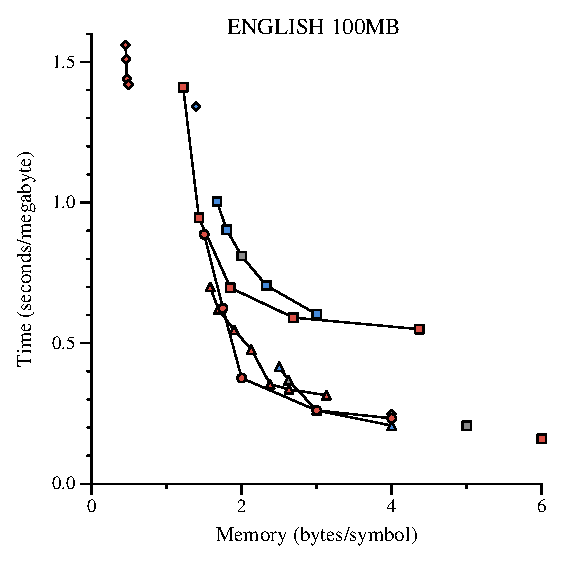
\includegraphics[width=60mm]{eng100Mb-new}
  \vspace{2mm}

  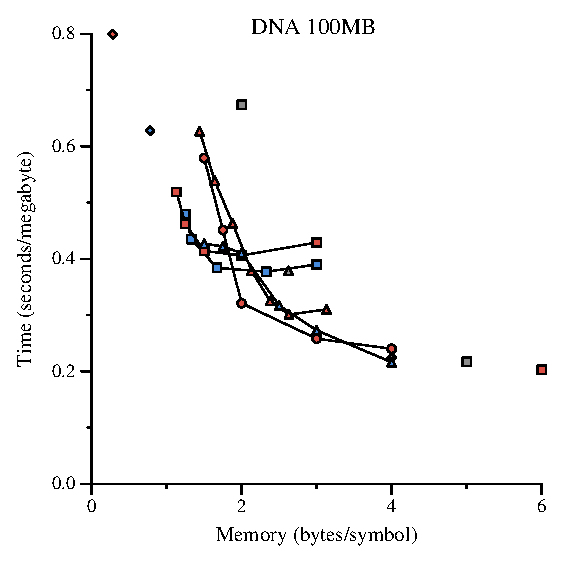
\includegraphics[width=60mm]{dna100Mb-new}
\end{textblock}

%\begin{textblock}{60}(130,165)
%  {\sffamily\normalsize{\color{sciorange}CONCLUDING REMARKS}}\vspace{1mm}\\
%  \footnotesize 
%\end{textblock}

\begin{textblock}{60}(130,185)
  \def\refname{\normalfont\sffamily\normalsize{\color{sciorange}REFERENCES}}
  \scriptsize\sffamily
  \bibliographystyle{abbrv}
  \bibliography{ibwt}
\end{textblock}

% Unfortunately, this template has no references. The official instructions seem to indicate that sans-serif font is used for the reference list.

\end{document}
